\documentclass[12pt]{article}
 \usepackage[margin=1in]{geometry} 
\author{Joshua Stephenson-Losey,
Keefer Sands,
Taylor Koth}
\usepackage{amsmath,amsthm,amssymb,amsfonts}
\usepackage{centernot}
\usepackage[table]{xcolor}
\usepackage{algpseudocode}
\usepackage{algorithm}
\usepackage{graphicx}
\usepackage{tikz}
\floatname{algorithm}{}
 
\newcommand{\N}{\mathbb{N}}
\newcommand{\Z}{\mathbb{Z}}
\renewcommand*{\proofname}{Solution}


\newenvironment{problem}[2][Problem]
{\begin{trivlist}
\item[\hskip \labelsep {\bfseries #1}\hskip \labelsep {\bfseries #2.}]}{\end{trivlist}}


\makeatletter
\renewcommand{\fnum@algorithm}{\fname@algorithm}
\makeatother

\begin{document}

 
\title{CSCI 432\\Homework 5}
\date{}
\maketitle

Assigned 10/31/2018, due by end of class (4:00 pm) on 11/26/2018. Marked questions (*) are graded for correctness. The remaining will be graded for effort. Please see the course website for details about expected effort.

You must follow the collaboration policy detailed on the course website. Please type solutions in an appropriate editor (\LaTeX, Word) so that I can review equations and proofs efficiently. 

\begin{problem}{1*}
Provide a graph that the vertex cover approximation algorithm always will find a suboptimal solution for.

In the graph below the vertex cover approximation algorithm will select six vertices, no matter the starting edge but the optimal solution is only four

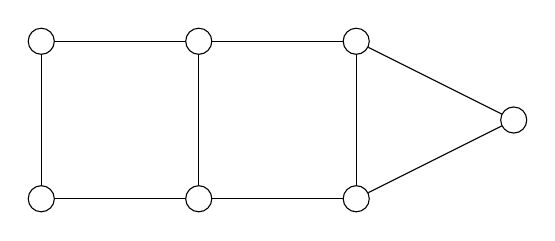
\begin{tikzpicture}
  [scale=.5,every node/.style={circle,draw}]
  \node (n4) at (4,10)  {};
  \node (n5) at (8,10)  {};
  \node (n1) at (12,8) {};
  \node (n2) at (8,6)  {};
  \node (n3) at (4,6)  {};
  \node (n6) at (0,10) {};
  \node (n7) at (0,6) {};
  
%   \node (n8) at (20,11)  {};
%   \node (n9) at (24,10)  {};
%   \node (n10) at (28,8) {};
%   \node (n11) at (24,6)  {};
%   \node (n12) at (20,5)  {};
%   \node (n14) at (16,10) {};
%   \node (n13) at (16,6) {};

  \foreach \from/\to in {n6/n7,n6/n4,n7/n3,n4/n5,n5/n1,n1/n2,n2/n5,n2/n3,n3/n4}
    \draw (\from) -- (\to);
    
%   \foreach \from/\to in {n14/n12,n14/n10,n14/n11,n8/n13,n8/n10,n8/n11,n9/n12,n9/n13,n10/n13,n10/n12,n13/n11,n14/n9}
    %  \draw (\from) -- (\to);

\end{tikzpicture}
\end{problem}


\begin{problem}{2*}
The Clique problem is: Given a graph, find the largest complete subgraph (i.e. largest subgraph where each pair of vertices share an edge). Given a graph $G$, the complement graph is the graph containing exactly the edges not in $G$. In other words, if $e=(u,v)$ is an edge in $G$, it is not in the complement graph. If $(x,y)$ is not an edge in $G$, then it is in the complement graph. An example of a graph and its complement is shown below. Show that a Clique of size $k$ in some graph $G$ is a Vertex Cover of size $|V|-k$ in the complement graph.

\begin{figure}[H]
\centering
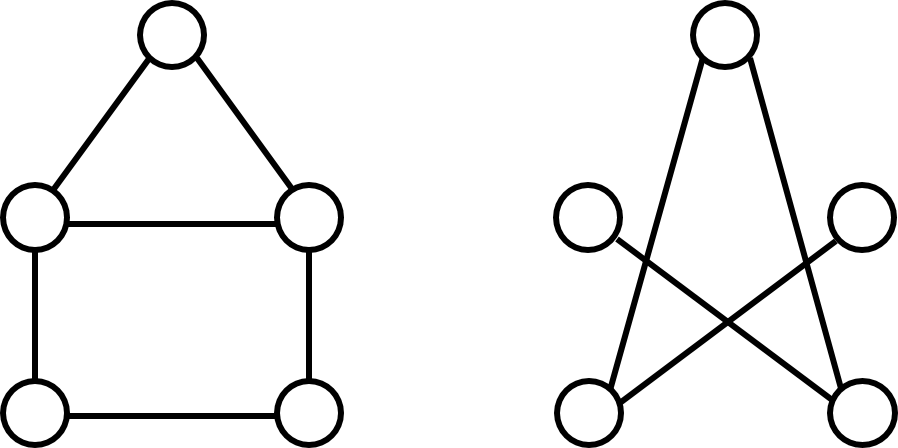
\includegraphics[scale=.5]{Homework5_comp.png}
\end{figure}

%in this graph the largest complete sub graph is the 3 vertex/ edge cycle that makes the triangle at the top of the graph. That makes the Clique size k = 3, the Vertex cover of the complement is size 2 or 5 - 3 where |V| = number of edges or 5

A Clique of size $k$ in a graph $G$ will be vertices in the complement graph $G'$ that do not share any edge with one another. This means that remaining vertices in the graph are connected to every edge of the complement graph and therefore are a Vertex Cover of the size $|V|-k$ where $|V|$ is every vertex of the graph and $k$ is the number of vertices from the Clique.
\end{problem}


\begin{problem}{3}
Since the complement of an optimal Vertex Cover gives a Clique of maximum size, does the $2$-approximation algorithm for Vertex Cover provide a constant ratio approximation algorithm for the Clique problem?

%in the graph above the 2 aprox algo run on the complement graph G' will result in 4 vertcies being chosen, two of which should be included in the Clique of G, which means the resulting aprox algo for the clique is alg > 1/a opt where a equals 3 since opt is 3 and alg is one

$OPT_{Vertex Cover} = |V| - k$ where $|V|$ is every vertex in a graph $G$ and $k$ is the number of vertices in the Clique of the complement, $G'$ as show in problem 2.

$ALG_{Vertex Cover} \le 2*OPT_{Vertex Cover} = 2(|V| - k) = 2(|V| - OPT_{Clique})$

$\therefore ALG_{Vertex Cover} \le 2(|V| - OPT_{Clique})$

This shows that the $2$-approximation algorithm for Vertex Cover provides a ratio approximation algorithm for the Clique problem that is based on the number of vertices in the graph which will not be constant for a general graph and is therefore not a constant ratio approximation.
\end{problem}


\begin{problem}{4*}
The Minimum Dominating Set problem is: Given a graph, find the smallest subset of the vertices such that each remaining vertex has a neighbor in the selected subset. Find an approximation algorithm for the Minimum Dominating Set problem (hint: Draw it out and see if it seems similar to a problem we studied in class).

%sounds like bipartite or more likely, set cover. maybe cuts?.... seems to be bipartite
Similar to Bipartite testing:

while vertices remain:

1) Put first vertex into set one

2) All its neighbors into set two

3) The neighbor of each neighbor into set one again

This will return a valid set of vertices where each vertex in set two has a neighbor in set one

\end{problem}


\begin{problem}{5}
Show up and participate in the workshop session on 11/9.
\end{problem}

\end{document}